\documentclass[a4paper]{article}
\usepackage[pdftex]{graphicx}
\usepackage[utf8]{inputenc}
\usepackage{enumerate}
\usepackage{amssymb}
\usepackage{icomma}
\usepackage{siunitx}
\sisetup{locale=DE} 
\usepackage{tikz}
\usepackage{href-ul}
\hypersetup{
	colorlinks=true,
	linkcolor=blue,
	urlcolor=blue}
\usepackage{geometry}
\geometry{a4paper, top=15mm, left=15mm, right=15mm, bottom=15mm,
	headsep=10mm, footskip=12mm}

\begin{document}
	
	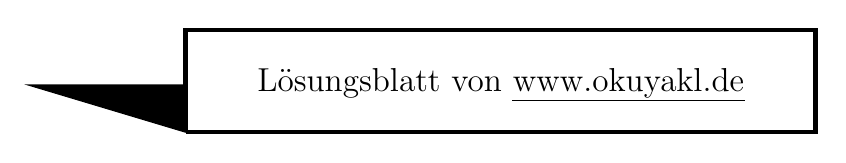
\begin{tikzpicture}(10,3)
		\draw[ultra thick](2,0) --(10,0) -- (10,1.3) --(2,1.3) -- (2,0);
		\draw[fill=black](2,0)-- (0,.6) -- (2,.6) -- (2,0);
		\node at (6,.6) {\large Lösungsblatt von \href{https://www.okuyakl.de}{www.okuyakl.de}};
	\end{tikzpicture}
	\vspace{0.5 cm}
	
{\bf Potenzen}

\begin{enumerate}[1.]
{\bf \item Vereinfache, wenn möglich, folgende Potenzen mit dem ersten Potenzgesetz $a^m \cdot a^n = a^{m+n}$}

\renewcommand{\arraystretch}{2}
\begin{tabular}{p{2.5 cm}p{2.5 cm}p{2.5 cm}p{2.5 cm}p{2.5 cm}p{2.5 cm}}
	a) $7^5$	&b) $3^5$  &c) $(-2)^7$ &d) $4^2$ &e) $\left({1\over 2}\right)^{11}$	&f) $(-8)$ \\
	g) $ 5^{-2}$ &h) $x^4$ &i) $ x^2$ &j) $2^{2x}$ &k) $2x^2$ &l) $3^{-8}$ \\
\end{tabular}

{\bf \item Vereinfache folgende Potenzen mit dem zweiten Potenzgesetz ${a^m \over a^n} = a^{m-n}$}

\renewcommand{\arraystretch}{2}
\begin{tabular}{p{2.5 cm}p{2.5 cm}p{2.5 cm}p{2.5 cm}p{2.5 cm}p{2.5 cm}}
	a) $7^2$	&b) $9^2$ &c) $6^{-7}$ &d) $4^8$ &e	$3^{-5}$&f) $2^{6}$\\
	g)  $x^6$ &h) $ 1$ &i)	$x^2$ &j) $2$&k) $3^{x}$&l) $x^{3}$\\
\end{tabular}

{\bf \item Wandle negative Potenzen in Brüche um und umgekehrt}

\renewcommand{\arraystretch}{2}
\begin{tabular}{p{2.5 cm}p{2.5 cm}p{2.5 cm}p{2.5 cm}p{2.5 cm}p{2.5 cm}}
	a) ${1\over 7}$	&b) $3^{-2}$ &c) $2$ &d) ${1\over 8^{3}}$&e) ${1\over x^{10}}$	&f) $x^{-12}$\\
	g) $(-1)$ &h) $5^{-3}$ &i) ${1\over 6^5}$ &j) ${1\over a^2}$ &k) ${1\over 2^{x}}$ &l) ${3\over 2}$ \\
\end{tabular}

{\bf \item Vereinfache folgende Potenzen mit dem dritten Potenzgesetz $(a^m)^n = a^{m\cdot n}$}

\renewcommand{\arraystretch}{2}
\begin{tabular}{p{2.5 cm}p{2.5 cm}p{2.5 cm}p{2.5 cm}p{2.5 cm}p{2.5 cm}}
	a) $2^6$	&b)  $7^{-4}$&c)  $4^{20}$&d)  $1,5^4$&e)	 $0,1^{-10}$&f)  $x^{-12}$\\
	g)   $1$&h)  $2^{2x}$ &i) $2^{2x}$&j)  $\left({5\over 6}\right)^{2}$&k)  $10^{-21}$&l)  $7^{12}$\\
\end{tabular}

{\bf \item Fasse zusammen nach den Regeln $a^nb^n = (ab)^n \qquad {a^n\over b^n} = ({a\over b})^n$}

\renewcommand{\arraystretch}{2}
\begin{tabular}{p{2.5 cm}p{2.5 cm}p{2.5 cm}p{2.5 cm}p{2.5 cm}p{2.5 cm}}
	a) $6^4 $	&b) $3^4$ &c) $10^{-7} $ &d) $5^2$ &e) $20^7 $ &f) $6^6$\\
	g) ${1\over 2^{10}}$ &h) $42^2$ &i) $7^4$	&j) $ \left({1\over 12}\right)^2$ &k) $2^2$ &l) ${3\over 2} $\\
\end{tabular}

{\bf \item Schreibe als Potenz mit möglichst einfacher Basis}

\renewcommand{\arraystretch}{2}
\begin{tabular}{p{2.5 cm}p{2.5 cm}p{2.5 cm}p{2.5 cm}p{2.5 cm}p{2.5 cm}}
	a) $3^4$ &b) $2^{-8}$ &c) $\left({1\over 2}\right)^6$ &d) $6^{20} $ &e)$\left({7\over 5}\right)^{2}$	&f) ${1\over 10^4} $\\
	g) $\left({8\over 6}\right)^6$ &h) $\left({2\over 3}\right)^{3}$&i)	$8^3$&j) $3^{-3}$ &k) $\left({2\over 8}\right)^8$&l) $\left({3\over 2}\right)^{3}$\\
\end{tabular}


{\bf \item Fasse zusammen, wenn möglich. Entscheide, welche Gesetze Du anwendest} 

\renewcommand{\arraystretch}{2}
\begin{tabular}{p{4 cm}p{4 cm}p{4 cm}p{4 cm}}
	a) $2^{10}$	&b) $7+7^2+7^3$ &c) $1$ &d) $2^{10}$\\
	e) ${1\over 7^2}$	&f) $12^2$ &g) $45^3$  &h) $2$\\
	i) $20^{-2}$ &j) $\left(3\over 2\right)^{10}$ &k) $3^4$ &l) $5^{3}$\\
\end{tabular}

{\bf \item Bestimme $x$}

\renewcommand{\arraystretch}{2}
\begin{tabular}{p{4 cm}p{4 cm}p{4 cm}p{4 cm}}
	a) $x=5$	&b) $x=8$ &c) $x=-2$ &d) $x=-3$ \\
	e) $x = {1\over 2}$ &f) $x =3$ &g) $x = -2$ &h) $x =0$ \\
\end{tabular}
\end{enumerate} 

\begin{center}
	\includegraphics[width=7 cm]{../../viecher/endcomic.pdf}
	
	Hier geht es zurück zum \href{https://www.okuyakl.de/math/m7pzgL113/aa113.pdf}{Aufgabenblatt}
\end{center}

\end{document}

